%==============================================================
%  Figura 5.6 - Arresto degli azionamenti 1 e 3 all'apertura
%  del cancello di protezione
%  Adattamento in italiano della Figura 5.6 dell'IFA Report 2/2017
%
%  Le campiture grigie evidenziano cio' che rientra nella funzione
%  di sicurezza: monitoraggio del cancello, logica e azionamenti 1 e 3.
%  L'azionamento 2 e' ritagliato in bianco perche' resta fuori dalla
%  funzione, pur essendo collegato alla stessa linea di comando.
%==============================================================
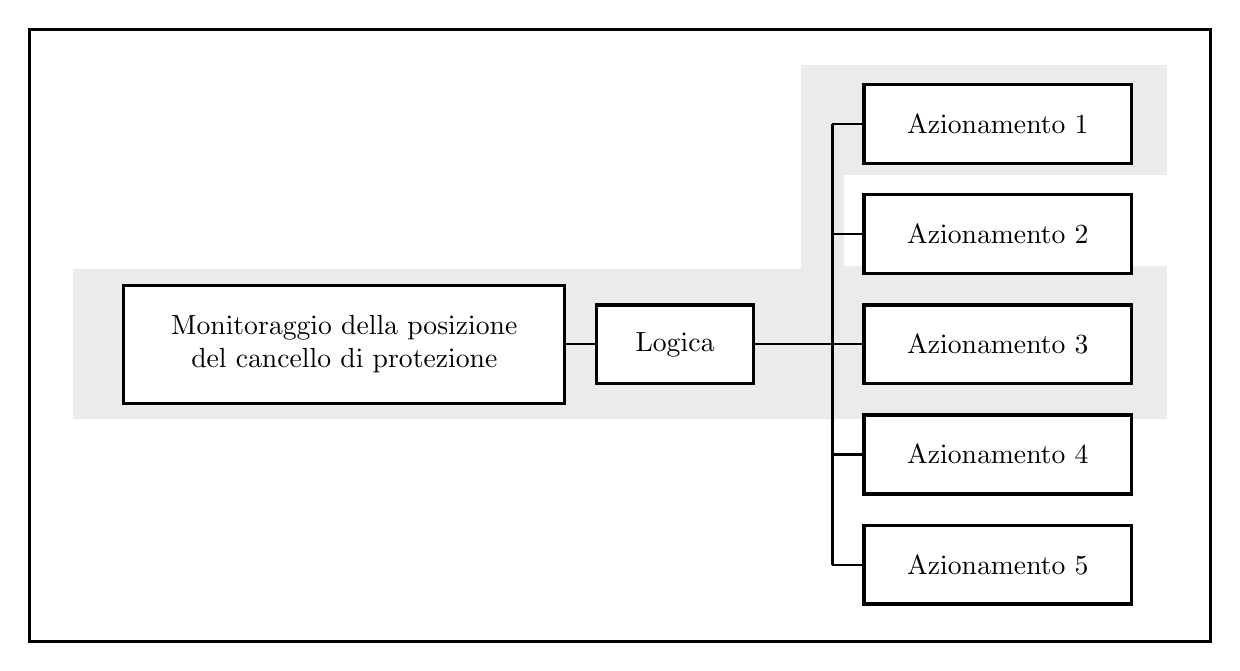
\begin{tikzpicture}[
  font=\normalsize,
  blocco/.style={draw=black, line width=1.2pt, fill=white, align=center,
                 inner sep=4pt, minimum height=1.0cm},
  azionamento/.style={blocco, minimum width=3.4cm},
  collegamento/.style={draw=black, line width=0.8pt}
]

% ---- campiture: prima le aree grigie, poi il ritaglio bianco --------
\fill[black!8] (-0.45,1.25) rectangle (13.45,3.15);   % fascia orizzontale
\fill[black!8] (8.80,3.15) rectangle (13.45,5.75);    % braccio verticale
\fill[white]   (9.35,3.20) rectangle (13.45,4.35);    % ritaglio: azionamento 2

% ---- blocchi -------------------------------------------------------
\node[blocco, minimum width=5.6cm, minimum height=1.5cm] (cancello) at (3.0,2.2)
  {Monitoraggio della posizione\\del cancello di protezione};
\node[blocco, minimum width=2.0cm] (logica) at (7.2,2.2) {Logica};

\node[azionamento] (az1) at (11.3, 5.0) {Azionamento 1};
\node[azionamento] (az2) at (11.3, 3.6) {Azionamento 2};
\node[azionamento] (az3) at (11.3, 2.2) {Azionamento 3};
\node[azionamento] (az4) at (11.3, 0.8) {Azionamento 4};
\node[azionamento] (az5) at (11.3,-0.6) {Azionamento 5};

% ---- collegamenti --------------------------------------------------
\draw[collegamento] (cancello.east) -- (logica.west);
\draw[collegamento] (logica.east) -- (az3.west);       % logica -> azionamento 3
\draw[collegamento] (9.2,5.0) -- (9.2,-0.6);           % linea di distribuzione
\draw[collegamento] (9.2,5.0) -- (az1.west);
\draw[collegamento] (9.2,3.6) -- (az2.west);
\draw[collegamento] (9.2,0.8) -- (az4.west);
\draw[collegamento] (9.2,-0.6) -- (az5.west);

% ---- cornice esterna -----------------------------------------------
\draw[draw=black, line width=1.2pt]
  ([shift={(-0.55,0.45)}]current bounding box.north west) rectangle
  ([shift={( 0.55,-0.45)}]current bounding box.south east);

\end{tikzpicture}
